%%%%%%%%%%%%%%%%%%%%%%%%%%%%%%%%%%%%%%%%%%%%%%%%%%%%%%%%%%%%%%%%%%%%%%%
%% Vorlage f�r Abschlussarbeiten                                     %%
%%-------------------------------------------------------------------%%
%% Datei:        Thesis.tex                                          %%
%% Beschreibung: Dies ist eine Vorlage f�r jegliche Abschlussarbeiten%%
%%               in der Wissenschaftlichen Einrichtung 4 an der      %%
%%               Universit�t der Bundeswehr M�nchen.                 %%
%% Autor: 	     Stefan Herrmann                                     %%
%%               Ferdinand Englberger                                %%
%% Datum:        26.01.2018                                          %%
%% Version:      1.0.5 05.12.2012 Stefan Herrmann                    %%
%%%%%%%%%%%%%%%%%%%%%%%%%%%%%%%%%%%%%%%%%%%%%%%%%%%%%%%%%%%%%%%%%%%%%%%

%%%%%%%%%%%%%%%%%%%%%%%%%%%%%%%%%%%%%%%%%%%%%%%%%%%%%%%%%%%%%%%%%%%%%%%
%% Dokumenteneinstellung und Laden von Paketen                       %%
%%%%%%%%%%%%%%%%%%%%%%%%%%%%%%%%%%%%%%%%%%%%%%%%%%%%%%%%%%%%%%%%%%%%%%%
\documentclass[
paper=A4,                      %a4paper,							% alle weiteren Papierformat einstellbar
%landscape,						% Querformat
12pt,								% Schriftgr��e (12pt, 11pt (Standard))
BCOR=1cm,							% Bindekorrektur, bspw. 1 cm
%DIVcalc,							% f�hrt die Satzspiegelberechnung neu aus
%											  s. scrguide 2.4
%oneside,							% einseitiges Layout
%twocolumn,						% zweispaltiger Satz
%openany,							% Kapitel k�nnen auch auf linken Seiten beginnen
%halfparskip*,				% Absatzformatierung s. scrguide 3.1
headsepline,					% Trennline zum Seitenkopf	
footsepline,					% Trennline zum Seitenfu�
%notitlepage,					% in-page-Titel, keine eigene Titelseite
%chapterprefix,				% vor Kapitel�berschrift wird "Kapitel Nummer" gesetzt
%appendixprefix,				% Anhang wird "Anhang" vor die �berschrift gesetzt 
%normalheadings,			% �berschriften etwas kleiner (smallheadings)
%idxtotoc,						% Index im Inhaltsverzeichnis
index=totoc,
%liststotoc,					% Abb.- und Tab.verzeichnis im Inhalt
listof=totoc,
%bibtotoc,						% Literaturverzeichnis im Inhalt
bibliography=totoc,
%leqno,								% Nummerierung von Gleichungen links
%fleqn,								% Ausgabe von Gleichungen linksb�ndig
%draft								% �berlangen Zeilen in Ausgabe gekennzeichnet
]
{scrbook}

%% Deutsche Anpassungen 
\usepackage[ngerman]{babel}
\usepackage[ansinew]{inputenc}
\usepackage[T1]{fontenc}
\usepackage{geometry}
\geometry{includehead,includefoot,inner=2.5cm,outer=2.5cm,top=2.5cm,bottom=2cm}
\usepackage{amsmath}
\usepackage{listings}
\usepackage{scrhack}  % Unterdr�ckt Deprecate Fehlermeldungen in Listings


%% Packages f�r Grafiken & Abbildungen 
\usepackage{graphicx} %%Zum Laden von Grafiken
\usepackage{subfigure} %%Teilabbildungen in einer Abbildung
\usepackage{float} %% F�r die Platzierung von Grafiken
\usepackage{placeins}

%% Sonstige Pakete 
\usepackage{eurosym}   % Euro Symbol
\usepackage{dsfont}    % Fonts f�r Zahlenbereiche


%% F�r das Erstellen von einem Index 
\usepackage{makeidx}
\makeindex 

%% Paket f�r die Erstellung von Links in der PDF Datei 
\usepackage[pdfborder={0 0 0}]{hyperref}

%% Paket f�r das Erstellen von zweispaltigen Abschnitten 
\usepackage{multicol}
\usepackage{tabularx}

%% Paket f�r die bessere Anpassung von Abst�nden zwischen W�rtern und Vermeidung von Zeilen die l�nger sind als die Textbreite
\usepackage{microtype}

%% Paket f�r das Einbinden von Quelltext
\usepackage{listings}
\usepackage{times}
\usepackage{pdfpages}

%% Einstellungen f�r Code Listings
\usepackage{color}
\definecolor{dkgreen}{rgb}{0,0.6,0}
\definecolor{gray}{rgb}{0.5,0.5,0.5}
\definecolor{mauve}{rgb}{0.58,0,0.82}
\definecolor{darkblue}{rgb}{0.1,0,1.0}
\definecolor{darkgreen}{rgb}{0.1,0.8,0.2}
 
\lstset{ %
  language=C++,                			% Die Sprache des Quelltexted
  basicstyle=\footnotesize,       % Die Textgr��e f�r den Quelltext
  numbers=left,                   % Wo sollen die Zeilennummern angezeigt werden.
  numberstyle=\tiny\color{gray},  % Stil f�r die Seitennummern
  stepnumber=1,                   % Schritt zwischen nummerierten zeilen. Bei eWie weit sind die Zeilennummern vom Code entfernt.
  backgroundcolor=\color{white},  % Hintergrundfarbe f�r den Quelltext
  showspaces=false,               % show spaces adding particular underscores
  showstringspaces=false,         % underline spaces within strings
  showtabs=false,                 % show tabs within strings adding particular underscores
  frame=single,                   % adds a frame around the code
  rulecolor=\color{black},        % if not set, the frame-color may be changed on line-breaks within not-black text (e.g. comments (green here))
  tabsize=2,                      % Die Gr��e f�r einen Tabulator
  captionpos=b,                   % Die Position der �berschrift. Hier b = Bottom
  breaklines=true,                % Automatischer Zeilenumbruch
  breakatwhitespace=false,        % sets if automatic breaks should only happen at whitespace
  title=\lstname,                 % show the filename of files included with \lstinputlisting;
                                  % also try caption instead of title
  keywordstyle=\color{blue},      % keyword style
  commentstyle=\color{dkgreen},   % comment style
  stringstyle=\color{mauve},      % string literal style
  escapeinside={\%*}{*)}          % if you want to add LaTeX within your code
}

\lstset{
    language=VHDL,language=VHDL,numbers=left,stepnumber=1,
    keywordstyle=\color{darkblue},
    commentstyle=\color{green},
    stringstyle=\color{darkgreen}
}

\usepackage{acronym}
\usepackage{csquotes}
\usepackage[backend=biber, abbreviate=false]{biblatex}
\addbibresource{bibliography/bibliography.bib}


%%%%%%%%%%%%%%%%%%%%%%%%%%%%%%%%%%%%%%%%%%%%%%%%%%%%%%%%%%%%%%%%%%%%%%%
%% Begin des Dokumentes                                              %%
%%%%%%%%%%%%%%%%%%%%%%%%%%%%%%%%%%%%%%%%%%%%%%%%%%%%%%%%%%%%%%%%%%%%%%%
\begin{document}

%% Titelseite
%%%%%%%%%%%%%%%%%%%%%%%%%%%%%%%%%%%%%%%%%%%%%%%%%%%%%%%%%%%%%%%%%%%%%%%
%% Vorlage f�r Abschlussarbeiten                                     %%
%%-------------------------------------------------------------------%%
%% Datei:        titlepage.tex                                       %%
%% Beschreibung: Titelseite f�r die Abschlussarbeit. Garantiert      %%
%%               ein einheitliches Design f�r alle Arbeiten am       %%
%%               Institut 4                                          %%
%% Autor: 			 Stefan Herrmann                                     %%
%% Datum:        30.06.2016                                          %%
%% Version:      1.0.3                                               %%
%% Version:      1.0.4                                               %%
%%%%%%%%%%%%%%%%%%%%%%%%%%%%%%%%%%%%%%%%%%%%%%%%%%%%%%%%%%%%%%%%%%%%%%%

\begin{titlepage}

\begin{center}

\begin{center}
	%%
\includegraphics{images/Uni_Logo_bw.jpg} 
	%% Alternativ auch in Farbe. Wichtig ist, dass nur eines von beiden einkommentiert wird.
	 
\includegraphics{images/Uni_Logo.jpg}
\end{center}

\vspace*{1cm}
\huge

%% Hier wird der Titel der Arbeit eingetragen
\textsc{Entwicklung einer Gestenerkennung mithilfe von Stereokameras mit ros}


\vspace{2cm}

\normalsize
%% Hier jeweils EINE der nachfolgenden Zeilen einkommentieren
\textsc{Masterarbeit\\[0.5\baselineskip] zur Erlangung des akademischen Grades\\[0.5\baselineskip] Master of Engineering (M. Eng.)}\\  
% \textsc{Masterarbeit\\[0.5\baselineskip] zur Erlangung des akademischen Grades\\[0.5\baselineskip] Master of Engineering (M. Eng.)}\\ 
% \textsc{Studienarbeit\\[0.5\baselineskip] im Rahmen des Studienganges\\[0.5\baselineskip] Applied Computer and Communication Technology}\\ 
% \textsc{Seminarstudie\\[0.5\baselineskip] im Rahmen des Studienganges\\[0.5\baselineskip] Computer Aided Engineering}\\  
\vspace{1cm}

\normalsize
Oliver Bosin %% Hier den eigenen Namen eintragen


\vspace{1cm}
Betreuer:\\
\vspace{0,3cm}
\begin{tabular}{ll}
		Prof. Dr. rer. nat. Norbert Oswald \\ %% ggf. Auskommentieren
\end{tabular}



\vspace{1cm}
Tag der Abgabe: 11.10.2020\\ %% Datum der Abgabe entsprechend anpassen.

\vspace{1cm}
Universit�t der Bundeswehr M�nchen\\
Fakult�t f�r Elektrotechnik und Technische Informatik\\
Institut f�r Verteilte Intelligente Systeme\\

\vspace{1cm}

Neubiberg, Oktober 2020 %% Hier den entsprechenden Monat und das Jahr vermerken

\end{center}

\end{titlepage}

\cleardoublepage

%% Vorspann
%%%%%%%%%%%%%%%%%%%%%%%%%%%%%%%%%%%%%%%%%%%%%%%%%%%%%%%%%%%%%%%%%%%%%%%
%% Vorlage f�r Abschlussarbeiten                                     %%
%%-------------------------------------------------------------------%%
%% Datei:        confirmation.tex                                    %%
%% Beschreibung: Enth�lt die Erkl�rung der selbstt�ndigen Arbeit     %%
%%               und die Einwilligung zur elektronischen Plagiats-   %%
%%               Pr�fung                                             %%
%% Autor: 			 Stefan Herrmann                                     %%
%% Datum:        28.11.2012                                          %%
%% Version:      1.0.1                                               %%
%%%%%%%%%%%%%%%%%%%%%%%%%%%%%%%%%%%%%%%%%%%%%%%%%%%%%%%%%%%%%%%%%%%%%%%

\newpage
\section*{Erkl�rung}
\textbf{gem�� Beschluss des Pr�fungsausschusses f�r die Fachhochschulstudieng�nge der UniBwM vom 25.03.2010}
\newline\newline
Hiermit versichere ich, dass ich die vorliegende Arbeit selbstst�ndig verfasst, noch nicht anderweitig f�r Pr�fungszwecke vorgelegt und keine anderen als die angegebenen Quellen und Hilfsmittel benutzt habe, insbesondere keine anderen als die angegebenen Informationen.
\newline\newline
Neubiberg, den 26. Juni 2019
\newline\newline\newline\newline
\rule{0.3\textwidth}{0.4pt} \newline
Oliver Bosin

\vspace{3cm}
\section*{Erkl�rung}
\textbf{gem�� Beschluss des Pr�fungsausschusses f�r die Fachhochschulstudieng�nge der UniBwM vom 25.03.2010}
\newline\newline
Der Speicherung meiner Masterarbeit zum Zweck der Plagiatspr�fung stimme ich zu. Ich versichere, dass die elektronische Version mit der gedruckten Version inhaltlich �bereinstimmt.
\newline\newline
Neubiberg, den 26. Juni 2019
\newline\newline\newline\newline
\rule{0.3\textwidth}{0.4pt} \newline
Oliver Bosin


\cleardoublepage %% Erkl�rungen gem Pr�fungsausschuss			
%%%%%%%%%%%%%%%%%%%%%%%%%%%%%%%%%%%%%%%%%%%%%%%%%%%%%%%%%%%%%%%%%%%%%%%
%% Vorlage f�r Abschlussarbeiten                                     %%
%%-------------------------------------------------------------------%%
%% Datei:        abstract.tex                                        %%
%% Beschreibung: Kurzzusammenfassung der Arbeit. Hierbei werden      %%
%%               Einleitung, Grundlagen, Messungen, Tests, Ergebnisse%%
%%               und ein Ausblick KURZ auf ca einer bis max zwei     %%
%%               Seiten zusammengefasst.                             %%
%% Autor: 			 Stefan Herrmann                                     %%
%% Datum:        05.12.2012                                          %%
%% Version:      1.1.1                                               %%
%%%%%%%%%%%%%%%%%%%%%%%%%%%%%%%%%%%%%%%%%%%%%%%%%%%%%%%%%%%%%%%%%%%%%%%

\chapter*{Abstrakt} %% Dieses Kapitel taucht nicht im Inhaltsverzeichnis auf.
\index{Abstrakt} %% Eintrag im Stichwortverzeichnis

Dieses Dokument dient zum Einen dazu, eine einheitliche Vorlage f�r alle Abschlussarbeiten im Institut 4 bereitzustellen. Zum Anderen wird es den Studenten hiermit vereinfacht eine umfassende Abschlussarbeit \index{Abschlussarbeit} anzufertigen, die gewissen Grundregeln f�r wissenschaftliche Arbeiten entspricht. Diese Vorlage ist nicht bindend. Es wird allerdings empfohlen, sich hieran zu halten. Auf diese Weise kann man sich auf den Inhalt und das Schreiben konzentrieren, ohne sich gro�e Gedanken �ber das Layout und die technische Umsetzung Gedanken machen zu m�ssen.

Das erste Kapitel einer Arbeit ist das Abstrakt. Auch wenn es chronologisch an erster Stelle steht, so wird es doch eigentlich zeitlich ganz am Ende geschrieben. Denn hier wird dem Leser ein umfassender �berblick \index{�berblick} �ber die Arbeit erm�glicht, ohne diese komplett lesen zu m�ssen. Alle wichtigen Punkte der Ausarbeitung m�ssen dabei aufgef�hrt werden. Beginnend mit einer Einleitung, den Grundlagen (bzw. Methoden), die Ergebnisse und Ausblick bzw. Diskussion. Die Kunst hierbei ist, dass sich \textbf{kurz} zu fassen. Ein Abstrakt sollte maximal zwei Seiten umfassen. 


 %% Abstrakt
\pagenumbering{Roman}	 
%%%%%%%%%%%%%%%%%%%%%%%%%%%%%%%%%%%%%%%%%%%%%%%%%%%%%%%%%%%%%%%%%%%%%%%
%% Vorlage für Abschlussarbeiten                                     %%
%%-------------------------------------------------------------------%%
%% Datei:        directories.tex                                     %%
%% Beschreibung: Umfasst Inhalts- Tabellen- und Abkürzungsverzeichnis%%
%% Autor: 			 Stefan Herrmann                                     %%
%% Datum:        28.11.2012                                          %%
%% Version:      1.0.0                                               %%
%%%%%%%%%%%%%%%%%%%%%%%%%%%%%%%%%%%%%%%%%%%%%%%%%%%%%%%%%%%%%%%%%%%%%%%

%% Festlegen der Tiefe des Inhaltsverzeichnisses
\setcounter{tocdepth}{2}

%% Inhaltsverzeichnis
\tableofcontents			

%% Tabellenverzeichnis
\listoftables				

%% Abbildungsverzeichnis
\listoffigures				
 %% Erzeugung von Verzeichnissen
\pagenumbering{arabic}           
%% Hauptteil der Arbeit 
%%%%%%%%%%%%%%%%%%%%%%%%%%%%%%%%%%%%%%%%%%%%%%%%%%%%%%%%%%%%%%%%%%%%%%%
%% Vorlage f�r Abschlussarbeiten                                     %%
%%-------------------------------------------------------------------%%
%% Datei:        introduction.tex                                    %%
%% Beschreibung: Einleitung f�r die Arbeit                           %%
%%               und ein Ausblick KURZ auf ca einer bis max zwei     %%
%%               Seiten zusammengefasst.                             %%
%% Autor: 			 Stefan Herrmann                                     %%
%% Datum:        28.11.2012                                          %%
%% Version:      1.0.0                                               %%
%%%%%%%%%%%%%%%%%%%%%%%%%%%%%%%%%%%%%%%%%%%%%%%%%%%%%%%%%%%%%%%%%%%%%%%

\chapter{Einleitung}
\index{Einleitung} %% Eintrag im Stichwortverzeichnis

\section{Motivation}
Nach dem Erfolg des Touchscreen ist sicher, dass die intuitive Bedienung von Technologien, einen gro�en Einfluss auf den Erfolg dieser hat.
Selbst in K�chenmaschinen, wie dem ''Thermomix'' von ''Vorwerk'', werden heutzutage Touchscreens verbaut. Da Roboter, f�r Industrie und auch f�r andere Nutzergruppen, immer wichtiger werden, stellt sich nun die Frage, wie eine intuitive Steuerung hier aussehen k�nnte. Bei den humanoiden Robotern oder Roboterarmen bietet sich hier die Gestensteuerung oder auch die Sprachsteuerung an. Mit einer Gestensteuerung k�nnte ein neuer Nutzer einen Roboterarm, nach nur einer kurzen Einweisung, mit Sicherheit ohne gr��ere Probleme steuern. Wenn eine intuitive Steuerung auch Roboter mehr Menschen n�her bringen k�nnte, dann w�rde dies die Forschung und Entwicklung, in dem Bereich der Robotik, beschleunigen. Im Falle vom Robot Operating System, w�rde, durch das gr��ere Interesse an der Robotik, die ROS-Community weiter anwachsen und die Weiterentwicklung von ROS vorantreiben. Innerhalb des Instituts 4 f�r Datentechnik und Schaltungstechnik, hat sich ROS bereits, als Basis f�r Projekte in der Robotik, bew�hrt. Unter Anderem wurden autonom fahrende Fahrzeuge, mit ROS als Basis, entwickelt. Die im Institut vorhandenen Fahrzeuge werden entweder durch Programmcode oder durch Fernsteuerungen gesteuert. Um diese M�glichkeiten der Steuerung, um die Gestensteuerung, zu erweitern, wird im Zuge dieser Bachelorarbeit eine Gestenerkennung, mit Hilfe von Stereokameras, mit ROS entwickelt und implementiert. 

\section{Aufgabenstellung}
Das Ziel dieser Bachelorarbeit ist es, mit Hilfe einer Stereokamera, mit ROS eine Gestenerkennung zu entwickeln und zu implementieren. Als sekund�r Ziel wird die Entwicklung eines ROS-Paketes, welches ein Beispiel f�r die Anwendung des Gestenerkennungssystems aufzeigt, angestrebt. Der Hauptzweck dieser Arbeit, neben der Entwicklung der Gestenerkennung, ist es, eine erste Grundlage, f�r Entwicklungen und nachfolgende Arbeiten, im Bereich der nat�rlichen Interaktion mit Robotersystemen zu legen. Wie sich die Gestenerkennung in die Umgebung von ROS einf�gt und wie sie in dieser Umgebung verwendet werden kann, sind Kernfragen dieser Grundlage. 


\section{Gliederung}
Die Arbeit besteht aus folgenden Kapiteln:

\begin{itemize}
\item \textbf{Kapitel 2 - Systemaufbau:}\\
Hier werden die Systemkomponenten aufgef�hrt und es werden jeweils kurze Erkl�rungen, zu jeder Komponente, gegeben. Ebenfalls wird hier Software und Hardware die verwendet wurde, aber nicht direkt zum Gestenerkennungssystem geh�rt, aufgef�hrt und kurz erkl�rt. Am Ende des Kapitels wird der gesamte Systemaufbau dargestellt und erkl�rt.
\item \textbf{Kaptiel 3 - Grundlagen:}\\
In diesem Kapitel werden grundlegende Funktionsweisen und Konzepte, der verwendeten Hardware und Software, erl�utert. Es wird hier auf die Stereokamera, das Framework ''OpenNI'', ROS und das Framework ''MoveIt!'' eingegangen.
\item \textbf{Kapitel 4 - Implementation des Gestenerkennungssystems mit ROS:}\\
Hier wird auf die Implementation des Gestenerkennungssystems eingegangen. Es wird ebenfalls auf die Inbetriebnahme und den Test des Systems eingegangen.
\item \textbf{Kapitel 5 - Implementation von Gestensteuerungen basierend auf dem Gestenerkennungssystem:}\\
In diesem Kapitel werden die entwickelten ROS-Pakete vorgestellt, welche Gestensteuerungen, die das Gestenerkennungssystem verwenden, implementiert haben. Es wird auf m�gliche Voraussetzungen, die Inbetriebnahme der Pakete und die Verwendung der Pakete eingegangen.
\item \textbf{Kapitel 6 - Diskussion:}\\
Im letzten Kapitel werden die Ergebnisse erl�utert und bewertet. Es wird zus�tzlich auf aufgetretene Probleme eingegangen. Zudem werden Empfehlungen, f�r weitere Arbeiten und Verbesserungen am System, gegeben. Am Ende wird noch ein allgemeiner Ausblick gegeben.
\end{itemize}




 % Einleitung
%%%%%%%%%%%%%%%%%%%%%%%%%%%%%%%%%%%%%%%%%%%%%%%%%%%%%%%%%%%%%%%%%%%%%%%
%% Vorlage f�r Abschlussarbeiten                                     %%
%%-------------------------------------------------------------------%%
%% Datei:        methods.tex                                         %%
%% Beschreibung: Methodenteil, der beschreibt welche Hard- oder      %%
%%               Software bereits vorhanden ist.                     %%
%%               und ein Ausblick KURZ auf ca einer bis max zwei     %%
%%               Seiten zusammengefasst.                             %%
%% Autor: 			 Stefan Herrmann                                     %%
%% Datum:        28.11.2012                                          %%
%% Version:      1.1.0                                               %%
%%%%%%%%%%%%%%%%%%%%%%%%%%%%%%%%%%%%%%%%%%%%%%%%%%%%%%%%%%%%%%%%%%%%%%%

\chapter{Systemaufbau}
\index{Systemaufbau} %% Eintrag im Stichwortverzeichnis
Der Aufbau, des gesamten Systems, l�sst sich in den Hardwareanteil und den Softwareanteil aufgliedern. Zuerst wird auf die verschiedenen Pakete und Treiber, die den Softwareanteil ausmachen, eingegangen und deren Zusammenspiel im Gesamtsoftwarekonzept erl�utert. Im zweiten Teil des Kapitels werden die Hardwarekomponenten des Systems vorgestellt. Hier wird als erstes die Aufgabe jeder relevanten Komponente beschrieben, um diese dann verst�ndlich in einen Kontext bringen zu k�nnen. Am Ende dieses Kapitels werden der Softwareanteil und der Hardwareanteil, im Gesamtkonzept, zu einer verst�ndlichen Darstellung des Systems zusammengef�gt.

\section{Software}
\index{Software}
In diesem Abschnitt wird die in dem Entwicklungsprozess verwendete und eingebundene Software vorgestellt. Dies soll einen ersten �berblick �ber den Entwicklungsprozess geben und das Gesamtsoftwarekonzept des Systems verst�ndlich darstellen. Die Installation und die genauere Verwendung, der hier genannten Software, ist integraler Teil des vierten Kapitels und wird somit hier nicht behandelt.

\subsection{Betriebsysteme}
Auf dem zur Entwicklung genutzten Rechner ist WINDOWS 10 als Betriebssystem installiert. Da ROS ein Framework f�r Linuxdistributionen ist, ist es notwendig ein Linux-Betriebssystem in einer virtuellen Maschine zu betreiben. Hierf�r wird eine virtuelle Maschine von ''VM-Ware' verwendet. 'In der virtuellen Maschine wird ein Ubuntu in der Version 16.04 LTS, welches in der WE4 laufend gepflegt und erweitert wird, betrieben. Unter dieser Ubuntu Version der WE4 ist das ROS-Framework, in der Version '''Kinetic Kame'', bereits installiert.
Bei der virtuellen Maschine von ''VM-Ware'' ist darauf zu achten, dass der USB-Kompatibilit�tsmodus  auf ''USB 3.0'' gesetzt ist, da sonnst Probleme mit USB-Ger�ten auftreten k�nnen.

\subsection{Integrierte Entwicklungsumgebungen}
F�r die Entwicklung von Software reicht in der Regel ein Texteditor und ein Compiler aus. Um diese Entwicklung komfortabler und �bersichtlicher zu gestalten werden integrierte Entwicklungsumgebungen verwendet. Hier sind normalerweise Texteditor, Compiler, Linker und weitere Programme in einer Anwendung integriert, um ein st�ndiges wechseln zwischen den Programmen zu vermeiden.

\subsection*{Eclipse}
Um Programme in der der Programmiersprache C/C++ zu entwickeln, wurde die integrierte Entwicklungsumgebung ''Eclipse''\cite{ECLIPSE} verwendet. Die verwendete Installation von ''Eclipse'' wurde innerhalb der WE4 mit dem ''Ubuntu'' Betriebssystem zusammen gepflegt. Weiterhin waren keine Anpassungen, der Konfiguration von ''Eclipse'', n�tig um Programme f�r das ROS-Framework darin zu entwickeln.

\subsection*{Keil}
Die integrierte Entwicklungsumgebung ''$\mu$-vision'' von ''KEIL'' wurde verwendet, um ggf. �nderungen an der Software, die auf dem Mikrocontrollerboard  l�uft, vorzunehmen.\cite{KEIL}
Auf das genannte Mikrocontrollerboard wird im Hardwareteil des Kapitels eingegangen.

\subsection{Robot Operating System}
Das ''Robot Operating System'' ist ein Quelloffenes und flexibles Framework, das darauf abzielt die Entwicklung von Software, f�r Robotersysteme, zu vereinfachen. Dazu stellt dieses Framework eine Sammlung von Tools, Bibliotheken und anderer Software zur verf�gung.\cite{ROS, KOUBAA2016} Unter ROS werden zur Entwicklung von Software die Programmiersprachen C/C++ und Python verwendet. Um die Konsistenz zu anderer Software die in der WE4 verwendet wird zu wahren, wurde f�r die im Zuge dieser Bachelorarbeit entwickelte Software die Programmiersprache C/C++ gew�hlt.
Auf den Aufbau und die Funktionen von ROS, wird im Grundlagenkapitel noch n�her eingegangen.

\subsection{OpenNI}
Um auf 3D-Sensoren wie Stereokameras zugreifen zu k�nnen, wurde unter ''Ubuntu'' das quelloffene Framework ''OpenNI'' verwendet. Es bietet API's um f�r 3D-Sensoren, RGB-Kameras, IR-Kameras und Audioeingabeger�te Anwendungen zu entwickeln.\cite{OPENNI} Im Zuge dieser Bachelorarbeit wurde hier die M�glichkeit von ''OpenNI''genutzt unkompliziert Treiber, f�r die genannten Ger�tetypen, einzubinden. Weiterhin ist dieses Framework notwendig, um Software die auf diesem basiert ausf�hren zu k�nnen. Dieses Framework ist als erster Baustein in dem Gesamtsoftwarekonzept des Systems zu sehen.

\subsection{SensorKinect}
Das Paket ''SensorKinect'' ist ein Modul f�r das Framework ''OpenNI''. Dieses Modul erm�glicht den Zugriff, �ber die API's von''OpenNI'', auf die Stereokamera ''Kinect'' von ''Microsoft''. \cite{SENSORKINECT}
Somit dient ''SensorKinect'' als Hardwaretreiber f�r die Stereokamera ''Kinect''. Als Modul f�gt sich ''SensorKinect'' in den Baustein ''OpenNI'' des Gesamtsoftwarekozeptes ein. Wird ein zum Treiber von ''PrimeSense'' kompatibler Sensor genutzt, ist die Installation von ''SensorKinect'' nicht erforderlich.\cite{OPENNI}

\subsection{Ros-Kinetic-OpenNI}
Um die Funktionen des Framework ''OpenNI'' auch in Verbindung mit ROS verwenden zu k�nnen, werden zus�tzlich mehrere ROS-Pakete, die im weiteren unter dem Namen''Ros-Kinetic-OpenNI'' gefasst werden sollen, ben�tigt.

\subsection{NITE} 
Das Paket ''NITE'' ist eine Middleware, die sich in die Infrastruktur des Framework ''OpenNI'' mit eingliedert. Diese Middleware erweitert die Funktionen von ''OpenNI'' unter anderem um das Tracking von Handbewegungen und K�rperbewegungen im ganzen.\cite{NITE,OPENNI}

\subsection{OpenNI Tracker}
Das ROS-Paket ''OpenNI Tracker'' greift auf die durch ''NITE'' implementierten Funktionen zu, um die Positionen von K�rpergelenken zu bestimmen und diese in ROS zur Verf�gung zu stellen.\cite{OPENNITRACKER}

\subsection{MoveIt!}
Mit ''MoveIt'' wurde ein weiteres Framework unter ROS genutzt. Das Framework ''MoveIt'' ist die ''State-Of-The-Art-Software'' f�r Navigationsplanung und Manipulationsplanung in der Robotik.\cite{MOVEIT,KOUBAA2016}

\subsection{Gesamtsoftwarekonzept}
In diesem Abschnitt wird das Gesamtsoftwarekonzept dargestellt und erkl�rt. Anhand der Abbildung 2.1, einer ''Abstract Layered View'', wird der Aufbau des Gesamtsoftwarekonzeptes erl�utert.

In diesem Kapitel wird Software beschrieben, welche f�r die Erf�llung der gestellten Aufgabe verwendet wurde: Also solche Anwendungen, die nicht selber geschrieben wurden. Hierzu z�hlen auch Programme, die von anderen Studenten in Abschlussarbeiten programmiert wurden. Es geht dabei darum, einen kurzen �berblick zu gew�hren. Es soll nicht jedes Fenster als Screenshot eingebunden werden. Wird beispielsweise die Anwendung Keil hier aufgef�hrt, so reicht ein kurzer Absatz mit Quellenverweis auf die Webseite. Wichtig in diesem Absatz ist nicht unbedingt, wie dieses Programm bedient wird, sondern vielmehr welche Version eingesetzt wurde, ob Zusatzmodule ben�tigt werden oder ob gewisse Funktionen deaktiviert werden m�ssen.

Im Rahmen dieser Vorlage werden jetzt zwei Programme und deren Installation erl�utert, weil diese f�r das Erstellen einer schriftlichen Ausarbeitung ben�tigt werden. Hierbei handelt es sich um eine Umgebung f�r das Latex Textsatzsystem, was die Bearbeitung dieser Vorlage erm�glicht.

\section{Hardware}
\index{Hardware}
In diesem Kapitel wird beispielsweise das Fahrzeug beschrieben. Aber auch eingesetzte Sensoren, Prozessoren etc. k�nnen hier jeweils ein Unterkapitel bekommen. Es ist darauf zu achten, dass hier nur der Vollst�ndigkeit halber eine Beschreibung eingef�gt wird. Dies soll einem Leser erm�glichen die Arbeit zu verstehen, der nicht hier an der WE arbeitet. Allerdings soll es nicht so ausarten, dass hier die komplette Dokumentation der einzelnen Bauteile abgeschrieben wird. In der K�rze liegt die W�rze. Auch ist darauf zu achten, dass die Dokumentation, Herstellerwebseiten etc. als Quellen angegeben werden.
 % Methodenteil
%%%%%%%%%%%%%%%%%%%%%%%%%%%%%%%%%%%%%%%%%%%%%%%%%%%%%%%%%%%%%%%%%%%%%%%
%% Vorlage f�r Abschlussarbeiten                                     %%
%%-------------------------------------------------------------------%%
%% Datei:        basics.tex                                         %%
%% Beschreibung: Grundlagenteil welcher verwendete Hard-   %%
%%               und Software n�her beschreibt.                            %%
%% Autor: 			 Stefan Herrmann                                     %%
%% Datum:        04.12.2012                                          %%
%% Version:      1.0.1                                               %%
%%%%%%%%%%%%%%%%%%%%%%%%%%%%%%%%%%%%%%%%%%%%%%%%%%%%%%%%%%%%%%%%%%%%%%%

\chapter{Grundlagen}
\index{Grundlagen} %% Eintrag im Stichwortverzeichnis
In diesem Kapitel wird auf die Grundlagen zu verwendeter Hard- und Software eingegangen. Dies soll Hintergrundinformationen zur gesamten Arbeit und speziell f�r die Ausf�hrungen im vierten Kapitel bereitstellen. Hierbei wird sich nur auf die wesentlichen Komponenten, f�r das Gesamtsystem, beschr�nkt.

\section{Stereokamera}
\index{Stereokamera}
Eine Stereokamera ist ein Kamerasystem,  dass zur Gewinnung von Tiefenbildern genutzt wird. Diese Tiefenbilder enthalten, im Gegensatz zu normalen Farbbildern, den Abstand einzelner Punkte zum Sensor der Kamera. Diese Kamerasysteme haben immer zwei optische Sensoren zur Bilderzeugung. Es gibt unter anderem Systeme mit zwei RGB-Sensoren sowie Systeme mit einem RGB-Sensor und einem Infrarotsensor.

\subsection{Typen}
Unter den Stereokameras gibt es verschiedene Typen, die sich in zwei Gruppen einteilen lassen: Diese Gruppen sind, Kameras mit passiven Verfahren und Kameras mit aktiven Verfahren. F�r diese Arbeit wurden die Beschreibungen auf die g�ngigsten Typen, von Stereokameras, begrenzt.

\subsection*{Embedded Stereo}
\index{Embedded Stereo}
Die ''Embedded Stereo'' Kameras nutzen das passive Stereoverfahren, um Tiefenbilder zu erzeugen. Diese Kamerasysteme haben meist zwei RGB-Sensoren um Bilder aufzunehmen, sowie einen eingebetteten Mikroprozessor oder FPGA, f�r die Berechnung von Tiefenbildern, integriert. Das passive Stereoverfahren ist an das menschliche Sehen angelehnt, bei dem aus zwei 2D-Bildern ein 3D-Bild gemacht wird. Das passive Verfahren, zur Erzeugung der Tiefenbilder, l�sst sich in mehrere Schritte aufteilen. Zu erst wird mit beiden RGB-Sensoren gleichzeitig ein Bild aufgenommen. Anschlie�end wird an beiden Bildern eine Merkmalextraktion durchgef�hrt. Diese Bildmerkmale, auch als ''Keypoints'' bezeichnet, lassen Unterschiede zu Ihrer Umgebung erkennen. Die gefundenen Bildmerkmale, beider Bilder, werden bei der Korrespondenzsuche miteinander verglichen. Nachdem die Korrespondenzsuche abgeschlossen ist, ist es noch notwendig falsche Korrespondenzen aus den Ergebnissen herauszufiltern. Mit den endg�ltigen korrespondierenden Bildmerkmalen kann nun, mittels Triangulation, die Entfernung zu diesem Merkmal im Bild errechnet werden.\cite{SCHMIEDECKE2009,MODROW2008}\\ Um den Prozessor des nutzenden Hauptsystems zu entlasten, werden die Berechnungen, f�r das beschriebene Verfahren, auf dem eingebetteten Mikroprozessor bzw. FPGA durchgef�hrt. Da der hohe Rechenaufwand auf eine erh�hte Leistungsaufnahme schlie�en l�sst, werden die ''Embedded Stereo'' Kameras nicht f�r mobile Systeme empfohlen. 

\subsection*{Time-Of-Flight}
\index{Time-Of-Flight}
Eine''Time-Of-Flight'' Kamera geh�rt zu den Kamerasystemen die aktive Verfahren, zur Generierung von Tiefenbildern, nutzen. Das von ''Time-Of-Flight'' Kameras genutzte Verfahren ist das Laufzeitverfahren. Bei dem Laufzeitverfahren wird ein Signal von der Kamera ausgesendet und die Zeit ermittelt wie lange das Reflektierte Signal gebraucht hat, um wieder an der Kamera aufzutreffen. Aus der Laufzeit t und Geschwindigkeit v des Signals kann, �ber die Formel $S =  v t$, direkt auf die Strecke S zum reflektierenden Objekt geschlossen werden. Als typische Emitter-Sensor Systeme, in dem Laufzeitverfahren, z�hlen Radar-, Ultraschall- und Infrarotsysteme.\cite{SCHMIEDECKE2009}\\ Die ''Time-Of-Flight'' Kameras nutzen in der Regel Infrarotsysteme. Die g�ngigen ''Time-Of-Flight'' Kameras haben meist einen RGB-Sensor, einen oder mehrere Infrarotemitter und einen Infrarotsensor verbaut. Aufgrund der hohen Ausbreitungsgeschwindigkeit von Licht, werden hohe Anforderungen an die Elektronik, zur Zeitmessung, gestellt. Unter anderem legt die kleinste messbare Zeitdifferenz $\triangle$t die maximale Tiefenaufl�sung $\triangle$R, mit der Formel $\triangle R = \frac{v \triangle t}{2}$ , fest.\cite{JIANGBUNKE1997} Durch diese hohen Anforderungen an die Elektronik, sind hochaufl�sende ''Time-Of-Flight'' Kameras kostenintensiv. Da hier Licht, im Infrarotbereich, detektiert wird, sind ''Time-Of-Flight'' Kameras nicht f�r Bereiche mit direkter Sonneneinstrahlung geeignet.\cite{BLANK2013} In Bereichen mit direkter Sonneneinstrahlung empfehlen sich stattdessen Kameras die auf passive Verfahren zur Tiefengewinnung zur�ckgreifen.

\subsection*{Infrarotmuster}
\index{Infrarotmuster}
Wie die ''Time-Of-Flight'' Kameras nutzen auch ''Infrarotmuster'' Kameras ein aktives Verfahren, zur Gewinnung von Tiefenbildern. Das Triangulationsverfahren, mit dem Ansatz des codierten Lichts, wird von den ''Infrarotmuster'' Kameras verwendet. Bei diesem Ansatz wird ein Infrarotmuster, mit bekanntem Code, in den Raum projiziert und mit einer Infrarotkamera aufgenommen. Somit sind, �ber den bekannten Code, alle vorher definierten Messpunkte im Bild eindeutig identifizierbar. Aufgrund der Kenntnis �ber die Position von Infrarotemitter und Infrarotkamera, kann f�r jeden Messpunkt der Abstand zur Kamera, �ber die Triangulation, errechnet werden.\cite{JIANGBUNKE1997,MODROW2008} Wie die ''Time-Of-Flight'' Kameras sind auch die ''Infrarotmuster'' Kameras, aufgrund der Verwendung von Infrarotlicht, nicht f�r Bereiche mit direkter Sonneneinstrahlung geeignet. Die f�r die Umsetzung des Gestenerkennungssystems dieser Arbeit genutzte Stereokamera, die ''Kinect'', ist eine ''Infrarotmuster'' Kamera. Somit ist das, in dieser Bachelorarbeit, entwickelte Gestenerkennungssystem nur f�r Innenbereiche geeignet.

\section{OpenNI}
\index{OpenNI}
Das Framework ''OpenNI'' soll in diesem Abschnitt, in seiner Funktion und seinem Aufbau, beschrieben werden. 

\subsection{Was ist OpenNI}
''OpenNI'' ist ein Framework, dass verschiedene Programmiersprachen erlaubt und f�r verschiedene Plattformen verf�gbar ist. Weiterhin definiert es API's zur Entwicklung von Anwendungen, die nat�rliche Interaktion, wie Sprache und Gesten, verwenden. Die API's von OpenNI bestehen aus mehreren Schnittstellen, zur Entwicklung von NI-Anwendungen. Der Hauptzweck von ''OpenNI'' ist es, eine Standard-API zur Verf�gung zu stellen, die eine Kommunikation mit folgenden Komponenten erm�glicht:

\begin{itemize}
\item optischen und akustischen Sensoren
\item Middleware, die Funktionen zur Verarbeitung von optischen und akustischen Sensordaten implementiert
\end{itemize}

''OpenNI'' liefert hierzu Schnittstellen die von den Sensorger�ten implementiert werden m�ssen sowie Schnittstellen die von der Middleware implementiert werden m�ssen. Durch diesen Ansatz werden Abh�ngigkeiten, zwischen Sensorger�ten und Middleware, vermieden. Dies erm�glicht es Anwendungen, ohne den Aufwand der Portierung, auf der Basis von verschiedenen Middleware's zu arbeiten. Des Weiteren bietet ''OpenNI'' die M�glichkeit, Anwendungen zu entwickeln die Sensorrohdaten verwenden, unabh�ngig vom Sensor der diese liefert.\cite{OPENNI}

\subsection{Module}
\index{Module}
Als Module werden Ger�tetreiber und Middleware bezeichnet, die im ''OpenNI'' Framework registriert wurden. Die folgenden Module werden von ''OpenNI'' unterst�tzt:\cite{OPENNI}

\subsubsection*{Sensormodule}
\begin{itemize}
\item 3D Sensor
\item RGB-Kamera
\item Infrarotkamera
\item Mikrofon
\end{itemize}

\subsubsection*{Middleware-Module}
\begin{itemize}
\item Middleware zur Ganzk�rperanalyse
\item Middleware zur Analyse der Handposition
\item Middleware zur Gestenerkennung
\item Middleware zur Analyse von Szenen in Bildern
\end{itemize}

\subsection{Kompatibilit�t und Verf�gbarkeit}
Die Entwickler von ''OpenNI'' garantieren volle R�ckw�rtskompatibilit�t\cite{OPENNI}. Dies bedeutet das Anwendungen, die auf Basis irgendeiner Version von ''OpenNI'' entwickelt wurden, mit neueren Versionen von ''OpenNI'' arbeiten k�nnen.\\
''OpenNI'' ist f�r folgende Betriebssysteme verf�gbar\cite{OPENNI}:

\begin{itemize}
\item Windows XP und aktueller
\item Linux Ubuntu 10.10 und aktueller
\end{itemize}

\section{ROS}
\index{ROS}
Dieser Abschnitt soll eine Einf�hrung in das Konzept, die Komponenten und das Vokabular von ROS geben. Diese Informationen sind, zum Verst�ndnis des vierten Kapitels, elementar. 
Die folgenden Punkte werden in dieser Einf�hrung behandelt:

\begin{itemize}
\item Was ist ROS
\item Konzept und Komponenten
\item Wichtige ROS-Befehle
\end{itemize}

\subsection{Was ist ROS}
Da ROS eine Vielzahl von Aufgaben eines Betriebssystems �bernimmt, aber als Umgebung ein Linux Betriebssystem ben�tigt, wird es oft als ''Meta-Betriebssystem'' bezeichnet. Die elementare Aufgabe von ROS ist es, eine Kommunikation zwischen Nutzer, Betriebssystem und externer Hardware bereitzustellen. Zur externen Hardware, mit der kommuniziert werden kann, z�hlen beispielsweise Sensoren, Kameras und Roboter. In dem ROS sich wie ein Betriebssystem verh�lt, bringt es den Vorteil der Hardwareabstraktion. Somit kann ein Nutzer einen Roboter steuern, ohne gro�e Kenntnis �ber dessen Hardware- und Softwaredetails zu haben. Als quelloffenes Framework, ist ROS f�r jeden frei verf�gbar. Dieser Ansatz wird auch bei den meisten ROS-Paketen verfolgt und diese unter der BSD-3-Lizenz ver�ffentlicht. Aufgrund dieser Voraussetzungen, werden neue Entwicklungen und neues Wissen, in der ROS-Community, schnell verbreitet. Aber auch f�r Unternehmen ist ROS interessant, da auch kommerzielle Produkte mit ROS entwickelt werden k�nnen. Hierf�r ist die einzige Bedingung, dass der Copyright-Vermerk der urspr�nglichen Software zitiert wird. \cite{FAIRCHILD2016,ROS}

\subsection{Konzept und Komponenten}
Das Konzept von ROS teilt sich in drei Konzeptschichten auf\cite{ROS}:

\begin{itemize}
\item ROS Dateisystem
\item ROS Computation Graph
\item ROS Community
\end{itemize}

\subsubsection*{ROS Dateisystem}
Das ROS-Dateisystem setzt sich aus folgenden Komponenten zusammen:

\begin{itemize}
\item Packages: In Paketen wird die Software in ROS organisiert.
\item Manifests: Im Manifest sind Metadaten �ber das Paket enthalten. Diese Manifests sind in XML geschrieben.
\item Stacks: Pakete, die gemeinsam eine Funktion bereitstellen, werden in Stacks zusammengefasst. 
\item Stack Manifest: Im Stack Manifest sind Metadaten �ber das Stack enthalten.\cite{FAIRCHILD2016,ROS}
\end{itemize}

\subsubsection*{ROS Computation Graph}
Das Netzwerk von Prozessen, die eine gemeinsame Aufgabe erf�llen, in ROS bildet den ''Computation Graph''. Die folgenden Komponenten versorgen den Graph mit Daten:

\begin{itemize}
\item Nodes: Als Knoten werden Prozesse in ROS bezeichnet, welche eine Aktion ausf�hren. Diese Knoten haben die M�glichkeit sich bei dem Master zu registrieren und untereinander zu kommunizieren. Die Verbindungsinformationen, zur Kommunikation untereinander, erhalten die Knoten vom Master. Hierf�r melden die Knoten dem Master welche Topics abonniert werden und auf welchen Topics Daten ver�ffentlicht werden. Knoten k�nnen auf verschiedene Arten gestartet werden. Zum einen �ber ein Terminalfenster durch ausgef�hrte Befehle, zum anderen als Teil eines Programms, geschrieben in Python oder C++.\cite{FAIRCHILD2016,ROS}

\item Master: Durch den Master wird die Kommunikation zwischen Knoten aufgebaut. Der Master bietet daf�r Namensdienste und Dienste zum registrieren an.  In Abbildung \ref{fig:Kommunikationsaufbau von Knoten} ist ein Kommunikationsaufbau beispielhaft dargestellt. Im ersten Schritt meldet sich der Knoten ''Camera'' beim Master an und informiert diesen dar�ber, dass, unter dem Topic ''images'', Bilder ver�ffentlicht werden. Im zweiten Schritt meldet sich der Knoten ''Imageviewer'' beim Master an und abonniert �ber diesen das Topic ''images''. Im dritten Schritt beginnt der Knoten ''Imageviewer'' die Bilder direkt �ber das Topic ''images'' zu empfangen.\cite{FAIRCHILD2016,ROS}

\begin{figure}
	\centering
		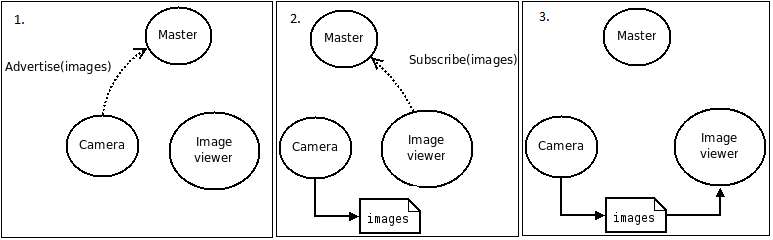
\includegraphics[width=0.85\textwidth]{images/basics/PublishSubscribe.png}
	\caption{Kommunikationsaufbau von Knoten}
	\label{fig:Kommunikationsaufbau von Knoten}
\end{figure}

\item Parameter Server: 
Der ''Parameter Server'' stellt eine geteilte Bibliothek von Parametern dar, welche innerhalb des Masters ausgef�hrt wird. Knoten k�nnen zur Laufzeit Parameter in dieser Bibliothek speichern und abrufen.

\item Messages: 
Wenn ein Knoten Daten unter einem Topic ver�ffentlicht, dann geschieht dies als sogenannte ''Message''.

\item Topics: 

\item Services: 

\item Bags: 

\end{itemize}

\subsubsection*{ROS Community}


\subsection{Wichtige ROS-Befehle}

\section{MoveIt!}
\index{MoveIt!} % Grundlagenteil
%%%%%%%%%%%%%%%%%%%%%%%%%%%%%%%%%%%%%%%%%%%%%%%%%%%%%%%%%%%%%%%%%%%%%%%
%% Vorlage f�r Abschlussarbeiten                                     %%
%%-------------------------------------------------------------------%%
%% Datei:        results.tex                                         %%
%% Beschreibung: Ergebnissteil der Arbeit der die erstellte Hard-    %%
%%               und Software beschreibt.                            %%
%% Autor: 			 Stefan Herrmann                                     %%
%% Datum:        04.12.2012                                          %%
%% Version:      1.0.1                                               %%
%%%%%%%%%%%%%%%%%%%%%%%%%%%%%%%%%%%%%%%%%%%%%%%%%%%%%%%%%%%%%%%%%%%%%%%

\chapter{Ergebnisse}
\index{Ergebnisse} %% Eintrag im Stichwortverzeichnis
Dieses Kapitel ist ganz der eigenen Arbeit gewidmet. Hier werden alle erzielten Ergebnisse und eigenen Arbeiten dokumentiert. An erster Stelle sind hier nat�rlich erstellte Platinen oder auch eigens erstellte Software zu nennen. Dar�ber hinaus werden hier aber auch durchgef�hrte Messreihen dokumentiert. Ergebnisse von Fahrtest, erstellte Umgebungskarten oder auch Screenshots der eigenen Software k�nnen ebenfalls hier aufgef�hrt werden. Allerdings werden hier noch keine Interpretationen hinsichtlich der Aufgabenerf�llung vorgenommen. Lediglich Beobachtungen und reine Fakten sind hier von Bedeutung. 

Zus�tzlich zu diesen allgemeinen Informationen zu dem Ergebnis-Kapitel werden in dieser Vorlage noch ein paar Informationen zu dem handwerklichen Vorgehen beim Erstellen einer schriftlichen Ausarbeitung aufgef�hrt. 

\section{Zitate}
\index{Zitate}
Grundlegend gilt: Alle Informationen, Aussagen, Bilder, Tabellen etc. die NICHT SELBER erstellt wurden, m�ssen �ber ein Zitat kenntlich gemacht werden \cite{Ufnalska2011,Kornmeier2012}. Bei uns wird in aller Regel nicht w�rtlich zitiert, also nicht 1-zu-1 abgeschrieben und in Hochkommata gesetzt. Vielmehr werden Informationen aus Artikeln, Webseiten, Datenbl�ttern oder �hnlichem �bernommen und sinngem�� wiedergegeben. Wird eine Quelle nicht deutlich gemacht, ist dies in der Regel ein Plagiat\index{Plagiat} \cite{Robert2007,Anderson1998}.

Es gibt sehr unterschiedliche Arten zu zitieren. Grundlegend wird in Geisteswissenschaften h�ufig in Form von Fu�noten zitiert. In der Naturwissenschaft ist ein nachgestelltes Literaturverzeichnis die Regel, so wie es auch in diesen Guidelines der Fall ist. Ein Zitat wird meist am Ende eines Satzes durch ein in eckige Klammern eingefasstes K�rzel angegeben. Dieses K�rzel kann numerisch durchnummeriert werden, IEEE Zitat Stil, oder aber Namens-K�rzel und Jahresangabe verwenden (bsp. [ENG2012]). Diese Vorlage nutzt im Wesentlichen den IEEE Zitierungs Stil.

Wenn Informationen aus dem Internet oder anderen Quellen verwendet werden, sind einige Punkte zu beachten. Nicht alles wird als zitierungsw�rdig betrachtet. So ist es beispielsweise un�blich Artikel aus Tageszeitungen oder �hnliches zu zitieren. Und auch Artikel aus Wikipedia sind nicht unbedingt guter Stil. Besser ist es sich B�cher oder wissenschaftliche Artikel zu dem Thema zu besorgen und diese zu referenzieren. �ber das Uni-Netz hat man Zugang zu mehreren online Quellen von wissenschaftlichen Artikeln. Wichtige Beispiele sind der IEEE Xplorer\index{IEEE Xplorer} \cite{IEEE}, SpringerLink\index{SpringerLink} \cite{Springerlink} oder auch die Unibibliothek \cite{UniBib}. Um ein paar Beispiele an die Hand zu geben, werden an dieser Stelle eine Bachelor-, eine Masterarbeit, ein Datenblatt sowie ein Skript referenziert \cite{Ruether2011,Solzbacher2011,LM2731,EmbSys}. 

\section{Bilder}
\index{Bilder}
Wenn die Bilder nicht selber erstellt wurden, dann m�ssen sie auf alle F�lle zitiert werden. Schwierig hierbei ist das Copyright. Um hier Problemen aus dem Weg zu gehen, wird empfohlen, keine Bilder aus dem Internet zu verwenden. Besser und unproblematischer ist es, selber einfache Zeichnungen zu erstellen. Bilder die im Institut~4 erstellt wurden, d�rfen verwendet werden, m�ssen aber mit Zitat (die Intranet Seite) gekennzeichnet werden.

Bilder aus wissenschaftlichen Artikeln d�rfen unter anderem abgedruckt werden. Hier ist es ratsam, sich im Vorfeld eine �Reprint Permission� vom Autor einzuholen. Viele Verlage haben eigene Vorgehen, um eine �Reprint Permissions� zu erteilen. Hier muss man sich vorher auf alle F�lle erkundigen ob man ein verwendetes Bild wirklich verwenden darf \cite{IEEEReprint,SpringerReprint}.

Auch die Platzierung von Bildern ist immer wieder missverst�ndlich. Generell sollten diese entweder ganz oben oder ganz unten auf der Seite zu finden und mit einer Bildunterschrift versehen sein. Bei der Verwendung von Latex wird dies automatisch erfolgen. Ganz wichtig ist, dass ein Bild immer im Text erw�hnt beziehungsweise erl�utert werden muss. Keine Bilder auff�hren, die nicht im Text Erw�hnung finden. Gerade Diagramme\index{Diagramm} o.�. m�ssen auch erl�utert werden. Ein SysML-Blockdiagramm\index{SysML}\index{Blockdiagramm}, ein Ablaufdiagramm\index{Ablaufdiagramm} oder ein Zustandsdiagramm\index{Zustandsdiagramm} (auch wenn sie nur im Anhang gezeigt werden) m�ssen textuell erl�utert und beschrieben werden. Bei Bildern von Robotern oder Sensoren reicht auch eine Erw�hnung in einem Halbsatz.

Als Beispiel zeigt die Abbildung \ref{fig:rumbler} das Kettenfahrzeug FTW-TV5 Rumbler\index{Rumbler} welches im Institut 4 f�r autonome Fahrversuche verwendet wird.

\begin{figure}
	\centering
		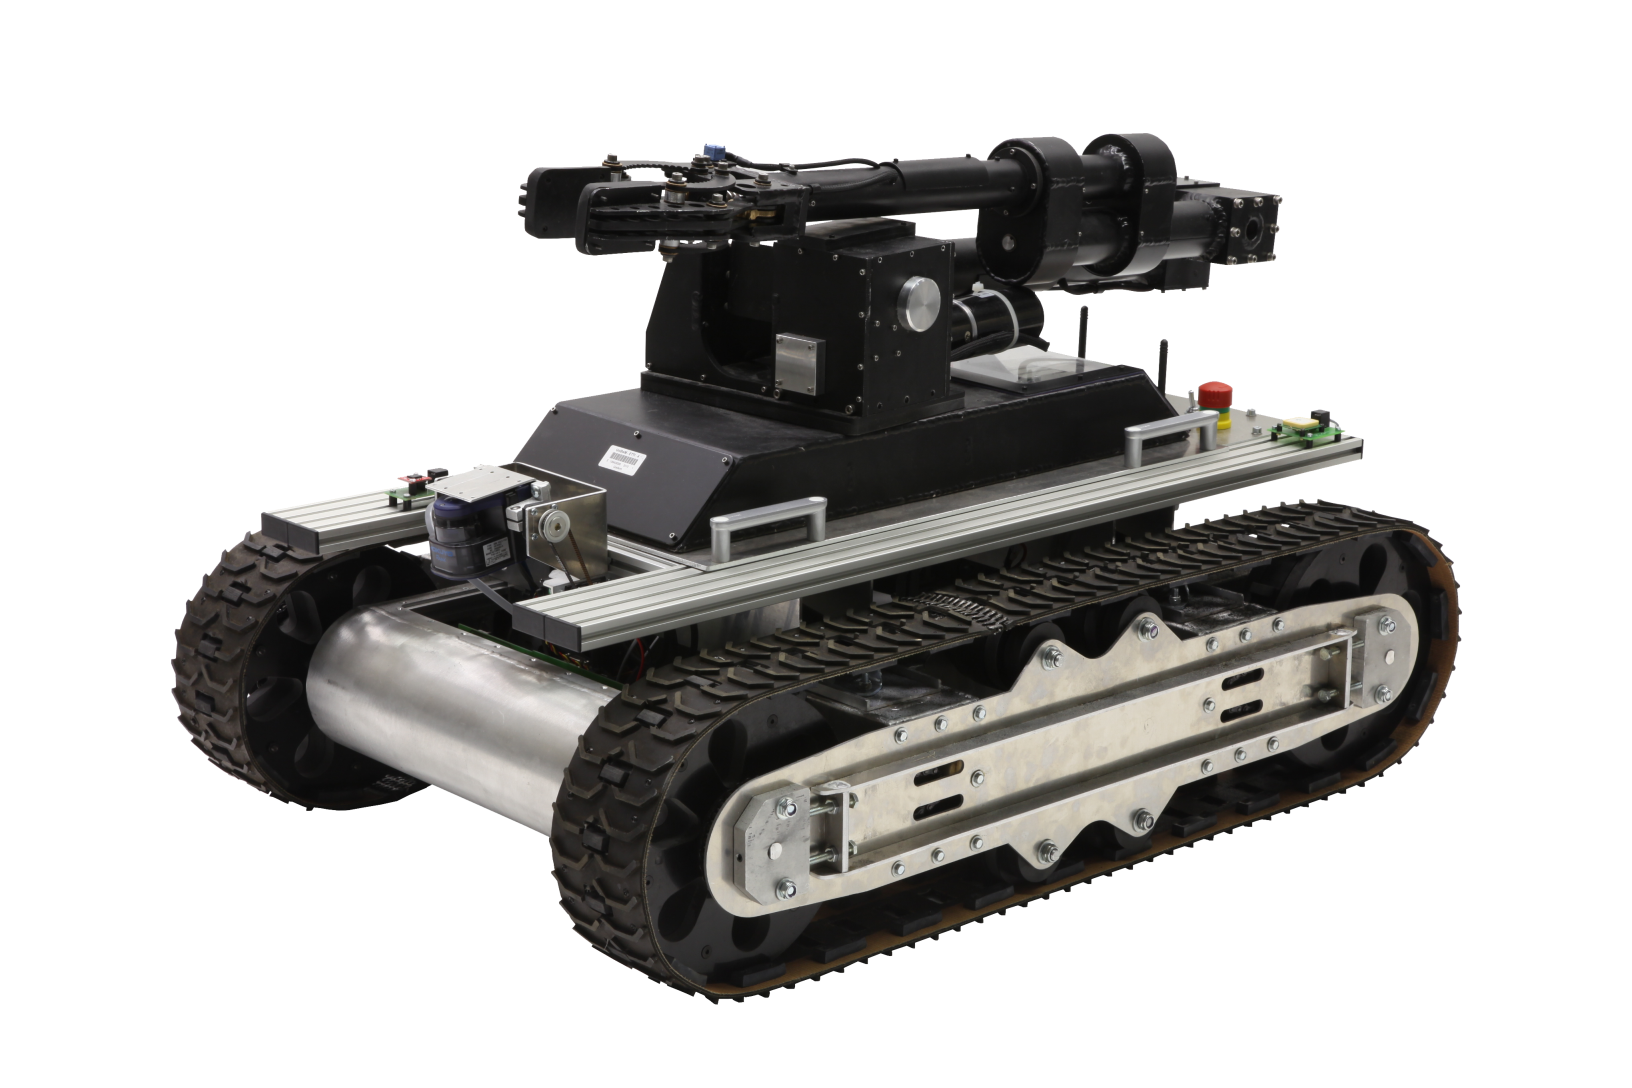
\includegraphics[width=0.6\textwidth]{images/results/rumbler.png}
	\caption{Autonomes Kettenfahrzeug des Instituts~4}
	\label{fig:rumbler}
\end{figure}

Sollen zwei Abbildungen nebeneinander platziert werden, so wird eine \textit{Subfigure} Umgebung verwendet. Auch andere Konstellationen mit mehr Bildern sind realisierbar sollen hier aber nicht weiter vertieft werden. Hierbei l�sst sich die komplette Abbildung referenzieren \ref{fig:subfigureexample} oder aber auch einzelne Unterabbildungen \ref{fig:panda}.

\begin{figure}
	\centering
		\subfigure[Panda]{
			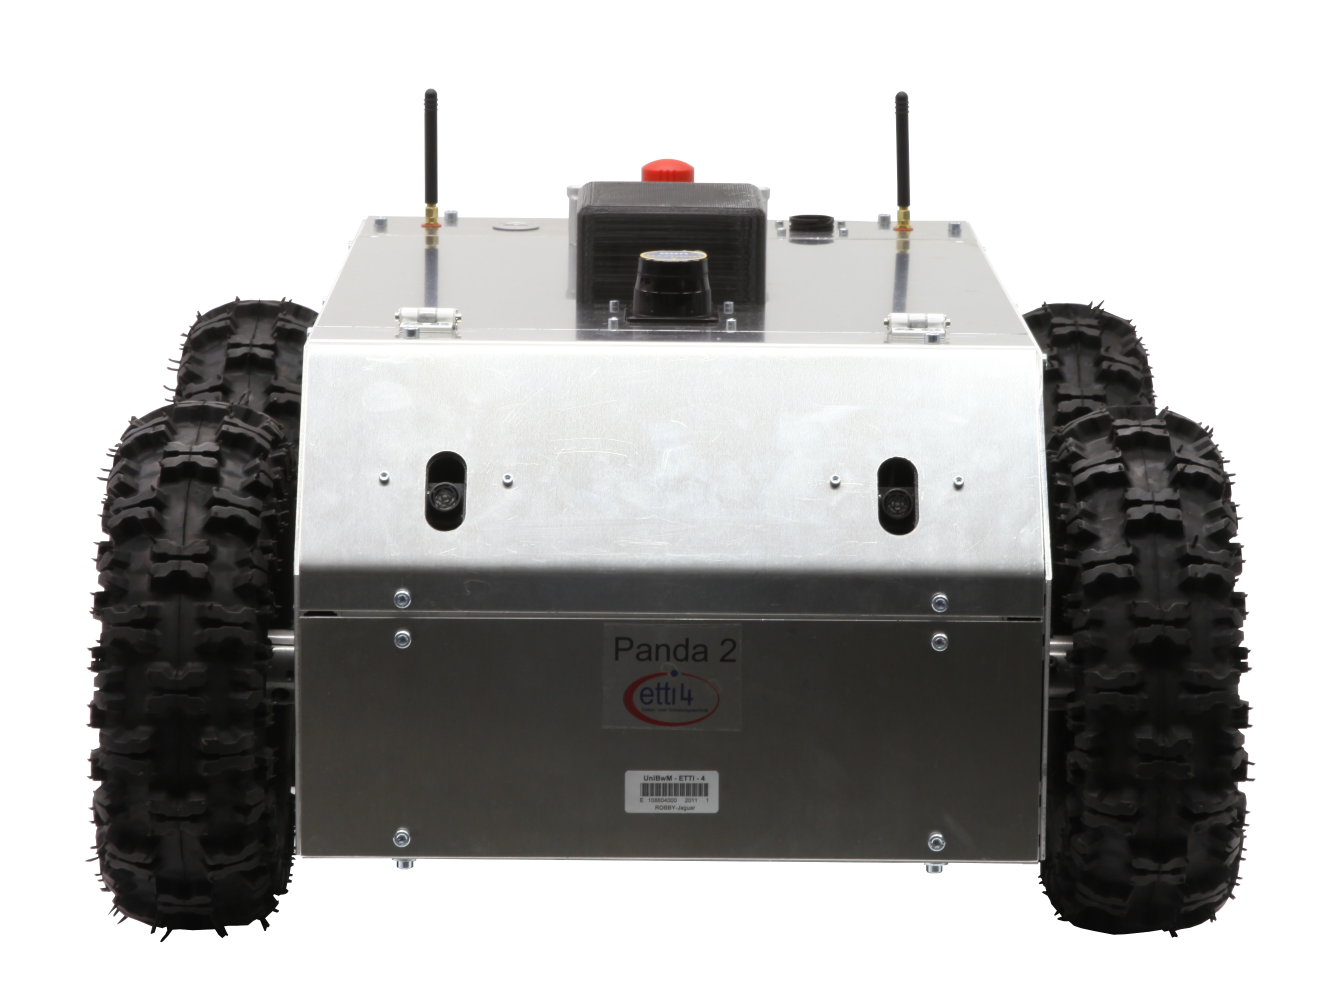
\includegraphics[width=0.4\textwidth]{images/results/panda.png}
			\label{fig:panda}
		}
		\subfigure[Bobby Car]{
			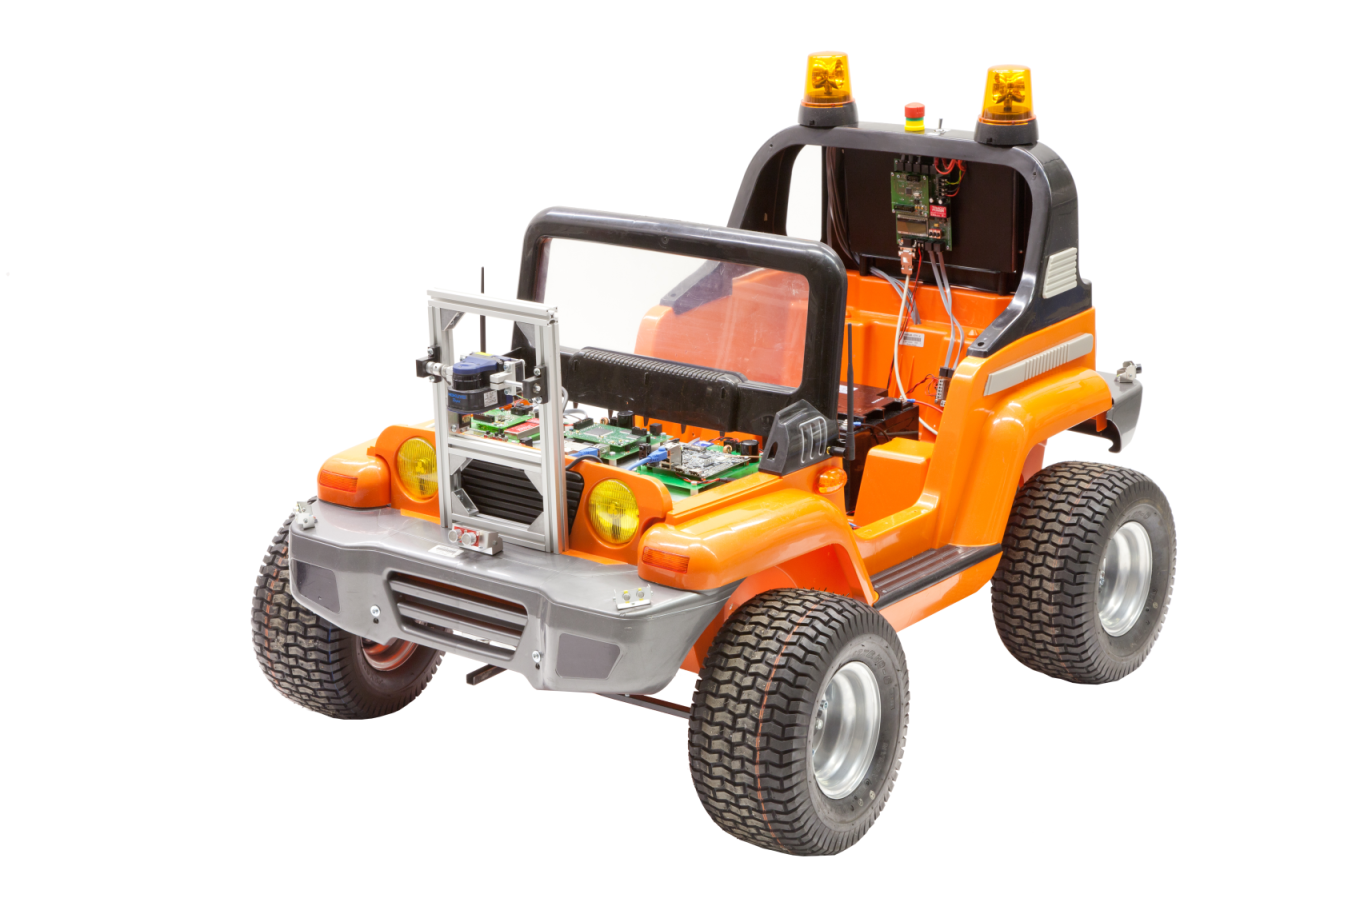
\includegraphics[width=0.4\textwidth]{images/results/bobbycar.png}
			\label{fig:bobbycar}
		}
	\caption{Fahrzeuge des Instituts~4.}
	\label{fig:subfigureexample}
\end{figure}


\section{Aufl�sung}
\index{Aufl�sung}
Werden eigene Diagramme und Skizzen erstellt, so ist auf eine gute Aufl�sung f�r den Druck zu achten. Die meisten Textsatzsysteme unterst�tzen leider keine Vektorgrafiken. Aber es ist m�glich die Abbildungen erst als Vektorgrafik\index{Vektorgrafik} zu erstellen (bsp. Mittel dem Open Source Tool Inkscape\cite{Inkscape}\index{Inkscape} und dann in einer hohen Aufl�sung in eine Rastergrafik\index{Rastergrafik} zu exportieren.

Auch das Erstellen von Abbildung aus Matlab\index{Matlab} heraus f�hrt immer wieder zu Problemen. H�ufigester Fehler ist eine zu niedrige Aufl�sung und zu kleine Schrift oder zu d�nne Linien. Hierbei sollte zun�chst einmal die Gr��e der Abbildung festgelegt werden. Dies kann unter Eigenschaften der Abbildung erfolgen, wie in Abbildung \ref{fig:matlab01} gezeigt. Danach k�nnen die Schriftarten und die Liniendicken entsprechend der schriftlichen Ausarbeitung angepasst werden. Danach sollte die Abbildung nicht einfach als Bild gespeichert, sondern Exportiert werden. Hierbei kann dann die Aufl�sung eingestellt werden, siehe Abbildung \ref{fig:matlab02}.

\begin{figure}
	\centering
		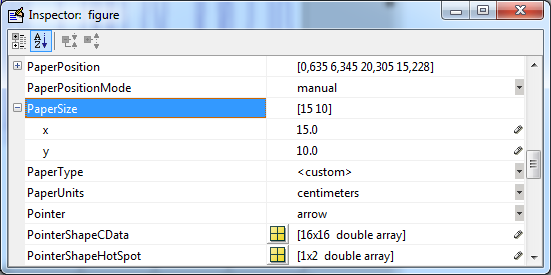
\includegraphics[width=0.50\textwidth]{images/results/matlab01.png}
	\caption{Einstellung der Gr��e f�r eine Matlab Abbildung.}
	\label{fig:matlab01}
\end{figure}


\begin{figure}
	\centering
		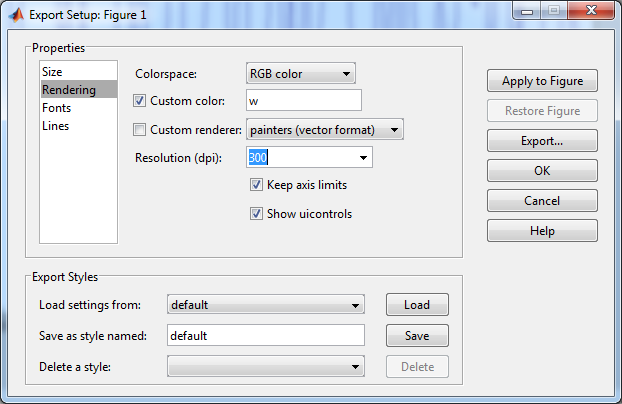
\includegraphics[width=0.60\textwidth]{images/results/matlab02.png}
	\caption{Einstellung der Abbildungs-Aufl�sung beim Exportieren aus Matlab heraus.}
	\label{fig:matlab02}
\end{figure}



\section{Farben}
\index{Farben}
Hierbei gilt: Weniger ist mehr. Nach M�glichkeit sind nur wenige oder gar keine Farben zu verwenden. Ausnahmen hierbei sind nat�rlich Fotografien. F�r alle selber erstellten Abbildungen gilt, dass diese im Zweifel besser und professioneller wirken, wenn man diese nur in Graustufen erstellt. Ein positiver Nebeneffekt ist, dass weniger Farbseiten beim Ausdruck anfallen. 


\section{Quelltext}
\index{Quelltext}
Hier im Institut~4 ist es die Regel, dass der Quelltext mittels dem Tool Doxygen dokumentiert wird. Insofern ist es nicht notwendig, den kompletten Quelltext im Text oder auch im Anhang aufzuf�hren. Trotzdem sollten \textbf{zentrale} Abschnitte im Text erl�utert werden. Beispielsweise ein komplizierterer Algorithmus oder �hnliches muss hier erw�hnt und beschrieben werden. Dies ist schlie�lich ein zentraler Teil der eigenen Arbeit. Dies dient zum einen der Dokumentation, da der Ablauf unter Umst�nden nicht aus den Dokumentierungen im Quelltext deutlich wird. Au�erdem muss die Arbeit auch f�r Au�enstehende verst�ndlich sein. Diese haben vielleicht keinen Zugang zur beigelegten CD.

Wird Quelltext in den Text eingebunden, so erfolgt dies �ber ein Listing. Ein Beispiel f�r eine sinnlose Funktion ist im Listing \ref{lst:Funktion} gegeben. Ein Beispiel daf�r, wenn eine externe Quelldatei eingebunden wird, ist im Listing \ref{lst:SN74x6541} zu finden.

\begin{tabular}{c}
\begin{lstlisting}[language=c, label=lst:Funktion, caption={Wichtige Funktion f�r das Programm}, linewidth=15cm]
	void do_something(int i , int y)
	{
		for (int index = 0; i < 100; i++)
		{
			i = i + index * y;
			if (mod(i, 2))
			{
				i = 1;
			}
			else
			{
				i = i*3;
			}
		}
	}
\end{lstlisting}
\end{tabular}

\begin{tabular}{c}
\lstinputlisting[language=vhdl, label=lst:SN74x6541, caption={Sourcecode SN74x6541}, linewidth=15cm]{source/SN74x6541.vhd}
\end{tabular}

\textbf{Nicht} ausreichend ist es, nur den Quelltext in der Arbeit aufzunehmen. Es ist sehr wichtig, dass auch die Funktion des Programmes erl�utert wird. So kann beispielsweise die Aufteilung in mehrere Tasks �ber ein Sequenzendiagramm dargestellt werden. Generell bieten sich Grafiken und Diagramme hier mehr an, als reiner Text. Ganz auf einen erkl�renden Text kann aber nicht verzichtet werden.


\section{Diagramme}
\index{Diagramme}
Bei gro�en Diagrammen (SysML\index{SysML}) stellt sich h�ufig die Frage, ob diese im Anhang oder im Text aufgef�hrt werden sollen. Wird ein bestehendes Diagramm lediglich wiedergegeben, so sollte dies in den Anhang. Ist das Diagramm aber ein zentraler Punkt der eigenen Arbeit, so sollte es auch im Text auftauchen. In beiden F�llen muss der Text den Diagramm-Inhalt erl�utern. Sehr gro�e Diagramme k�nnen auch in mehrere Abbildungen aufgesplittet werden.


\section{Layout}
\index{Layout}
Auch wenn es dem eigenen Design-Empfinden besser passt, die Arbeit einseitig zu drucken: Es empfiehlt sich, einen doppelseitigen Druck zu verwenden. Die Arbeit wird nicht nach Gewicht bewertet und so kann an Druckkosten gespart werden. Auch hat man somit mehr Informationen auf einen Blick. Bei der Verwendung dieser Vorlage muss doppelseitig gedruckt werden, weil ansonsten die Seitennummerierung mal auf der linken und mal auf der rechten Seite des Blattes erscheint.


\section{Sprachliches}
\index{Sprache}
Nicht jedem liegt das Schreiben von spannenden Texten. Lassen Sie den Text von jemandem lesen, der von der Thematik keine Ahnung hat. Im Zweifel eher k�rzere S�tze verwenden. Nicht zu lange Schachtels�tze erzeugen. Lieber Aufz�hlungen verwenden. 

Ein h�ufig wiederkehrender Punkt sind sogenannte "`Weichmacher"', die in einer wissenschaftlichen Arbeit nach M�glichkeit vermieden werden: "`sollen, sollte, k�nnte, w�re m�glich, etc."'. Definitiv schreiben. Der Roboter muss folgende Aufgaben erf�llen. Dies wiederstrebt einem in der Regel, wenn man wei�, dass vielleicht noch nicht alles hundertprozentig funktioniert. Diese Weichmacher hinterlassen aber den Eindruck, dass der Autor sich seiner Arbeit nicht so sicher ist oder auch nicht davon �berzeugt ist.


\section{Abk�rzungen}
\index{Abk�rzungen}
Ein Abk�rzungsverzeichnis ist nicht verpflichtend. Aber jede eingesetzte Abk�rzung, muss beim ersten Auftauchen erl�utert werden. Dies kann als Fu�note, in Klammern oder auch im Text erfolgen. Als Beispiel sei hier SysML\footnote{System Modelling Language} aufgef�hrt.


\section{Tabellen}
\index{Tabellen}
Zu Tabellen gelten die gleichen Regeln wie auch f�r Abbildungen. Jede Tabelle muss im Text erl�utert oder zumindest erw�hnt werden. Auch sollte darauf geachtet werden, dass die Tabellen �bersichtlich bleiben und nicht �berladen werden.  Als Beispiel listet Tabelle die unterschiedlichen Diagramme der \textit{System Modelling Language} auf.


\begin{table}
	\centering
		\begin{tabular}{|p{0.4\textwidth}|p{0.6\textwidth}|}
			\hline
			\textbf{Diagramm} & \textbf{Anmerkung} \\ \hline \hline 
			System Context Diagram & Gibt einen �berblick �ber das System und die Interaktion mit der Umwelt.\\
			Use Case Diagram & Anwendungsf�lle, also das was mit dem System gemacht werden kann.\\
			Block Definition Diagram & Aufteilung in System und Subsysteme.\\
			Internal Block Definition Diagram & Schnittstellen von Subsystemen zueinander.\\
			Requirements Diagram & Anforderungen an das System.\\
			Package Diagram & Wird hier nicht ben�tigt.\\
			State Machine & Zust�nde die das System annehmen kann.\\
			Allocations & Wird hier nicht ben�tigt.\\
			Parametric Diagram & Wird hier nicht ben�tigt.\\
			Sequence Diagram & Ablauf von Funtkionen und Nachrichtenfl�ssen.\\
			Activity Diagram & Abfolge von Aktivit�ten im System.\\ \hline
		\end{tabular}
	\caption{Diagrammarten der System Modelling Language}
	\label{tab:DiagrammartenDerSystemModellingLanguage}
\end{table}


\section{Formeln}
\index{Formeln}
Formeln k�nnen zum einen direkt inline im Text oder abgesetzt eingef�gt werden. Wird sich f�r eine abgesetzte Formel entschiede, dann sind diese zu nummerieren, um sie im Text referenzieren zu k�nnen. Alle etwas komplizierteren Formeln sollten abgesetzt werden, um das Schriftbild �bersichtlich zu halten. Einfache Zusammenh�nge, wie beispielsweise $x_i = \cos{(i - 1)}$, st�ren das Schriftbild aber nicht weiter. Als Beispiel f�r eine abgesetzte Formel sei auf Formel \ref{eq:Formel} oder \ref{eq:Formel2} verwiesen.

\begin{align}
f(x_{k,i}, x_{k+1,i})=
\begin{cases}
1	& \text{falls} \hspace{1cm} (-x_{k,i} \cdot x_{k+1,i}) > 0 \wedge |x_{k,i} - x_{k+1,i}| > \text{Schwellwert}\\
0 & \text{sonst}
\end{cases}
\label{eq:Formel}
\end{align}

\begin{align}
A = 
\left(
\begin{array}{ccc}
a   &   b    &    c \\
d   &   e    &    f \\
g   &   h    &    i 
\end{array}
\right)
\label{eq:Formel2}
\end{align}
 % Ergebnissteil
\chapter{Diskussion}
\index{Diskussion} %% Eintrag im Stichwortverzeichnis
Im Zuge dieser Bachelorarbeit wurde ein Gestenerkennungssystem, mithilfe einer Stereokamera, in ROS entwickelt und implementiert. Dieses Ziel wurde, nach Schwierigkeiten mit veralteten Rechner und nicht aktueller ROS-Distribution, erfolgreich erreicht. Dar�ber hinaus wurde, mit zwei entwickelten ROS-Paketen, gezeigt, wie dieses Gestenerkennungssystem in ROS eingesetzt werden kann. Damit ist das Ziel, eine Grundlage f�r weitere Arbeiten und neue Interaktionsm�glichkeiten mit Robotersystemen zu schaffen, ebenfalls als erf�llt zu betrachten.
In diesem Kapitel werden die erzielten Ergebnisse, die aufgetretenen Probleme und die gewonnenen Erkenntnisse zusammenfassend erl�utert.\\
Das entwickelte und implementierte Gestenerkennungssystem ist funktionsf�hig und bildet eine gute Grundlage, f�r zu entwickelnde Applikationen. Das System bindet die verwendete Stereokamera ein, greift auf die durch diese gelieferten Daten zu und verarbeitet die erhaltenen Daten. Die verarbeiteten Daten werden in ROS zur Verf�gung gestellt und mit Hilfe dieser ein ''Skelett-Tracking'' erm�glicht. Das ''Skelett-Tracking'' wurde in den beiden entwickelten Paketen verwendet. Das System verf�gt, �ber das verwendete ''Skelett-Tracking'' hinaus, �ber weitere Funktionen, wie zum Beispiel die Erkennung von bestimmten Bewegungsabl�ufen. Zu Beginn der Entwicklung traten mehrere Probleme auf. Das erste Problem, welches viel Zeit kostete, wurde durch die virtuelle Maschine ausgel�st. Das Linux-Betriebssystem, welches in der virtuellen Maschine lief, konnte nur fehlerhafte Daten von der Stereokamera empfangen. Dies Problem wurde durch eine Anpassung der USB-Kompatibilit�tseinstellungen, von USB 2.0 auf USB 3.0, gel�st. Doch auch nach dieser Anpassung, wurde die Verbindung zu Stereokamera noch in Einzelf�llen unterbrochen. Um diese Art von Problemen zu vermeiden, sollte, bei weiteren Arbeiten oder Weiterentwicklungen am System, wenn m�glich auf eine native Linux-Installation zur�ckgegriffen werden. Eine native Linux-Installation ist ebenfalls f�r die gesamte Systemperformance positiv. Als zweites, aber kleineres, Problem zeigte sich, dass Alter der verwendeten ROS-Distribution. Durch das, im Mai 2016, zur�ckliegende Ver�ffentlichungsdatum von ''ROS Kinetic Kame'' und durch die Tatsache, dass es bereits seit Mai 2018 eine neue ROS-Distribution gibt, wurden verschiedene Komponenten des Gestenerkennungssystems, f�r ''ROS Kinetic Kame'', nicht mehr weiterentwickelt. Aufgrund dieser Tatsache, musste auf nicht aktuelle Versionen der Komponenten zur�ckgegriffen werden. Dies f�hrte zu einem Mehraufwand in der Entwicklung, aber nicht zu einer feststellbaren Einschr�nkung des Systems. Bei der entwickelten Gestensteuerung, f�r den Roboterarm, traten Probleme bei der Bewegungsplanung auf. Es wird hier nur unzuverl�ssig ein Bewegungspfad gefunden. Das Problem wurde auf die Berechnung der inversen Kinematik und den verwendeten Pfadplaner, innerhalb von ''MoveIt!'', eingegrenzt. Der Versuch eine L�sung, innerhalb der verf�gbaren Zeit, zu finden, war leider nicht erfolgreich. Mit der hier durchgef�hrten Eingrenzung des Problems, wird die Suche nach einer L�sung jedoch kein gro�es Problem darstellen.\\
Als erste Erkenntnis steht am Ende dieser Arbeit, dass die nat�rliche Interaktion, des Menschen mit technischen Systemen, viel Potential ins sich tr�gt. Durch weitere Arbeiten in diesem Bereich, werden ganz sicher neue Ans�tze entstehen und somit die Interaktion mit Robotern, neu definiert werden. Als zweite Erkenntnis steht, dass ROS, durch sein modulares Konzept und die daraus resultierende einfache Integration neuer Hardware und Software, eine passende Umgebung f�r weitere Entwicklungen in diesem Bereich darstellt. 

\section{Ausblick}
\index{Ausblick}
Diese Bachelorarbeit bietet eine Grundlage f�r weitere Entwicklungen, in dem Bereich der nat�rlichen Interaktion mit Robotersystemen. Die, zu Beginn der Arbeit, gesteckten Ziele wurden erreicht, jedoch sind weitere Arbeiten an dem System notwendig. Als erstes ist hier die Migration, des Systems, auf die aktuellste ROS-Distribution zu nennen. Im Zuge der Migration werden Aktualisierungen, an den Systemkomponenten, durchgef�hrt werden m�ssen. Gegebenenfalls wird es auch notwendig sein, dass Komponenten des Systems ausgetauscht werden m�ssen. Neben den Aktualisierungen der Software, bietet sich der Austausch der ''Kinect'', durch eine aktuellere und leistungsst�rkere Stereokamera, an. Durch einen Austausch lassen sich, durch die h�here Genauigkeit aktueller Stereokameras, neue Funktionen implementieren. Durch neue Funktionen lassen sich wiederum neue Anwendungen, f�r das Gestenerkennungssystem, finden. Aus der Entwicklung der Gestensteuerung, f�r den Roboterarm, ging hervor, dass die Bewegungsplanung noch nicht zufriedenstellend funktioniert. Hier empfiehlt es sich die Pakete ''rob\_arm\_small'' und ''rob\_arm\_small\_hw\_interface'' zu �berarbeiten. Hier sollte das Hauptaugenmerk auf die Kinematik , die verwendeten Bewegungsplaner und auf die verwendete URDF-Datei gelegt werden.\\
Das Konzept, dass hinter dem Gestenerkennungssystem steht, erm�glicht es auch andere Sensoren, neben Stereokameras, zu integrieren. Somit k�nnen, in Weiterentwicklungen des Systems, verschiedene Sensoren miteinander kombiniert werden. Die Implementation einer Spracherkennung w�re beispielsweise eine M�glichkeit. Neben den genannten Weiterentwicklungen,  gibt es die M�glichkeit, dass System in andere Projekte zu integrieren. Zum Beispiel eine Personenfolgefunktion, f�r mobile Robotersysteme, k�nnte damit integriert werden. Abgesehen von so spezifischen Verwendungen, wie einer Personenfolgefunktion, kann auch nur die Umgebungswahrnehmung, von bestehenden Robotersystemen, erweitert werden. 


Es hat sich bew�hrt, einen Ausblick zu geben, was weiterhin verbessert werden kann. Welche �nderungen an der Software sind noch notwendig, welche Hardware-Umbauten w�ren hilfreich etc. Das ist gerade f�r uns wichtig, wenn wir weiter Arbeiten f�r dieses Fahrzeug o.�. anbieten. % Diskussion und Ausblick

%% Nachspann der Arbeit 
%%%%%%%%%%%%%%%%%%%%%%%%%%%%%%%%%%%%%%%%%%%%%%%%%%%%%%%%%%%%%%%%%%%%%%%
%% Vorlage f�r Abschlussarbeiten                                     %%
%%-------------------------------------------------------------------%%
%% Datei:        appendix.tex                                        %%
%% Beschreibung: Weitere Informationen, Schaltpl�ne und Quelltext    %%
%% Autor: 			 Stefan Herrmann                                     %%
%% Datum:        03.12.2012                                          %%
%% Version:      1.0.1                                               %%
%%%%%%%%%%%%%%%%%%%%%%%%%%%%%%%%%%%%%%%%%%%%%%%%%%%%%%%%%%%%%%%%%%%%%%%
\appendix
\chapter{Quellcode}
\index{Quellcode}
\lstinputlisting[language=C++, caption={move\_group\_interface.cpp}]{images/results/move_group_interface.cpp}
\lstinputlisting[language=C++, caption={gesture\_control.cpp}]{images/results/gesture_control.cpp}


\chapter{Arbeitsaufwand}
\index{Arbeitsaufwand}

\begin{figure}[H]
	\centering
		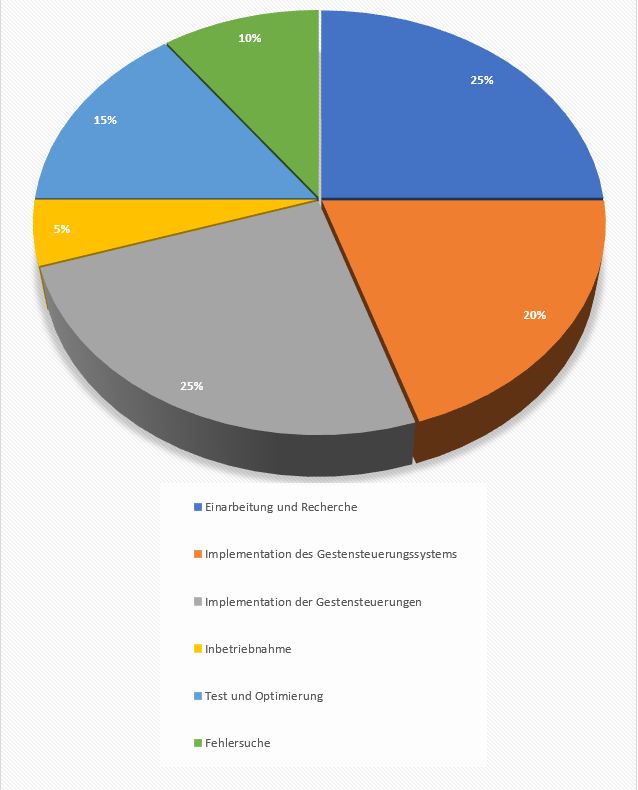
\includegraphics{images/appendix/DiagrammArbeitsaufwand.png}
	\caption{Arbeitsaufwand}
	\label{fig:arbeitsaufwand}
\end{figure}




 % Der Anhang

\printbibliography[heading=bibintoc]
\newpage
\small
\printindex





\end{document}
